\documentclass[12pt,table,xcolor={dvipsnames}]{beamer}
\usetheme{Pittsburgh}
\usecolortheme{seagull}
%\usepackage[utf8]{inputenc}
\usepackage{fontspec}
\usepackage{amsmath}
\usepackage{listings}
\usepackage{multirow}
\usepackage{amsfonts}
\usepackage{amssymb}
\usepackage{graphicx}
\author{Design and Verification of Security Protocols and Security Ceremonies}
\title{\vspace{-.7cm}Cryptographic Primitives \\\vspace{-.7cm} Asymmetric Cryptography}
%\setbeamercovered{transparent} 
\setbeamertemplate{navigation symbols}{} 
%\logo{
\includegraphics[scale=0.015]{Brasao_UFSC.png}
\includegraphics[scale=0.2]{brasao_PPGCC.jpg}} 
\institute{Programa de Pós-Graduacão em Ciências da Computacão \\ Dr. Jean Everson Martina} 
\date{\vspace{-1cm}August-November 2016} 
\subject{} 
\usebackgroundtemplate{
\includegraphics[width=\paperwidth,
height=\paperheight]{../reusable_images/fundo_UFSC.png}}
\begin{document}

{
\usebackgroundtemplate{
\includegraphics[width=\paperwidth,
height=\paperheight]{../reusable_images/fundo_capa.png}}
\begin{frame}
\titlepage

\includegraphics[scale=0.3]{../reusable_images/brasao_PPGCC.jpg}
\end{frame}
}

\begin{frame}{Message Authentication Codes}
\begin{itemize}
\item They couple the idea of an integrity checking functions with shared key crypto-system;\pause
\item They are also length reducing functions;\pause
\item They are publicly known;\pause
\item And ease of computation.
\end{itemize}
\end{frame}

\begin{frame}{MAC Functions' Properties}
\begin{itemize}
\item Given $n$ pairs $(m_1, MAC_k(m_1))$,..., $(m_n, MAC_k(m_n))$ find a new  pair $(m, MAC_k(m))$ efficiently and with non negligible probability is unlikely;\pause
\item Output should be a length-reduction function;\pause
\item The key should control the mapping between the Domain and Image of the MAC function, but not determine its spread.
\end{itemize}
\end{frame}

\begin{frame}{MAC Construction}
\begin{itemize}
\item There are basically two mains ways of producing secure MAC systems:\pause
\begin{itemize}
\item Symmetric CBC-MAC;\pause
\item CMAC;\pause
\item Hash based HMAC;
\end{itemize}
\end{itemize}
\end{frame}

\begin{frame}{CBC-MAC Mode of Encryption}
\begin{columns}
\column{.5\textwidth}
\begin{center}
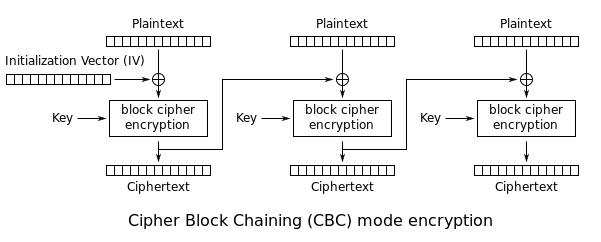
\includegraphics[scale=.25]{../Lecture_2/CBC_encryption.png};
\end{center}
\column{.5\textwidth}
\begin{itemize}
\item It is basically the application of CBC over input data;\pause
\item Instead of keeping all the blocks we just keep the last one;\pause
\item Its length is determined by block size;\pause
\item IV is fixed.
\end{itemize}
\end{columns}
\end{frame}

\begin{frame}{Security of CBC-MAC}
\begin{itemize}
\item Secure for messages of a fixed number of blocks assuming the block cipher is Pseudo-Random Permutation;\pause
\item Not secure with variable lengths;\pause
\item Needs to be used with one key to each message length or do length pre-pending;
\end{itemize}
\end{frame}

\begin{frame}{CMAC}
\begin{columns}
\column{.5\textwidth}
\begin{center}
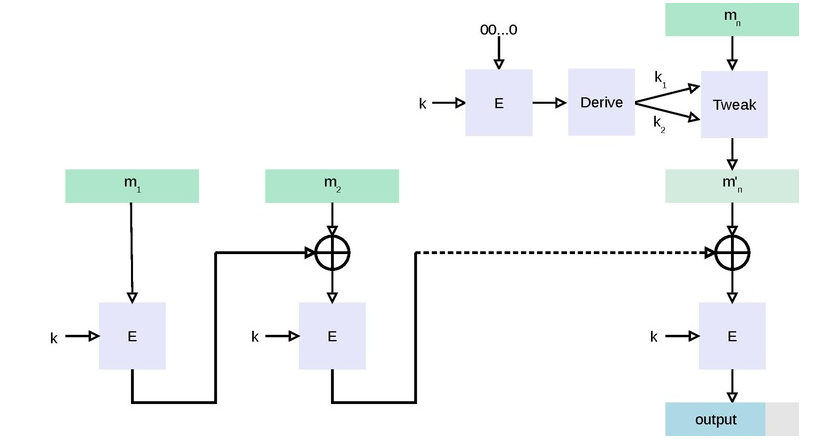
\includegraphics[scale=.22]{OMAC.png}
\end{center}
\column{.5\textwidth}
\begin{itemize}
\item It is a NIST standard for doing MAC with symmetric cyphers;\pause
\item Efficiently addresses the security deficiencies of CBC-MAC;\pause
\item Derives 2 keys to cypher the last block;
\end{itemize}
\end{columns}
\end{frame}

\begin{frame}{HMAC Properties}
\begin{itemize}
\item Use available hash functions without modification;\pause
\item Preserve the original performance of the hash function;\pause
\item Use and handle keys in a simple way;\pause
\item Allow easy replacement of the underlying hash function;\pause
\item Have a well-understood analysis of the strength of the authentication mechanisms;
\end{itemize}
\end{frame}

\begin{frame}{HMAC}
\begin{center}
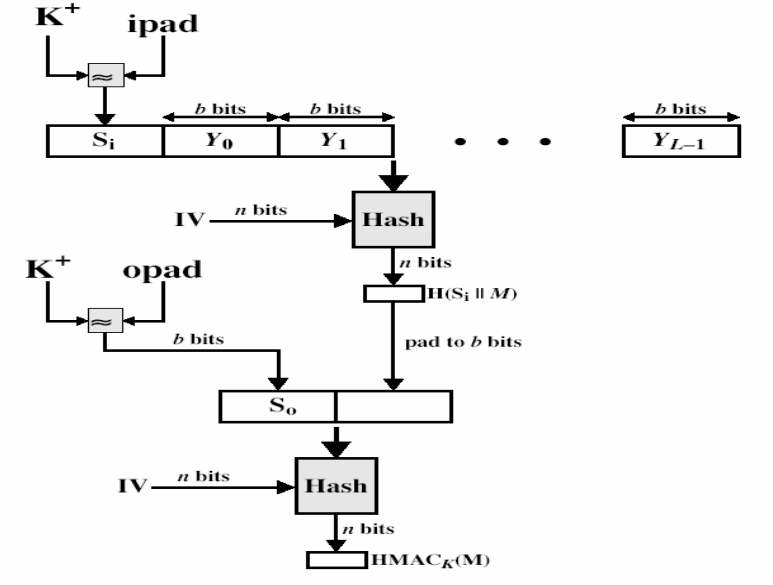
\includegraphics[scale=.33]{HMAC.png}
\end{center}
\end{frame}

\begin{frame}{Security of HMAC}
\begin{itemize}
\item Security of HMAC relates to that of the underlying hash algorithm;
\item If used with a secure hash functions and according to the specification (key size, and use correct output), no known practical attacks;
\end{itemize}
\end{frame}

\begin{frame}{Asymmetric Cryptography}
\begin{itemize}
\item Appeared on the 1970s. First classified by GCHQ and later publicly by Diffie and Helmann's work;\pause
\item Comes to solve the secure distribution channel on symmetric cryptography;\pause
\item A user has two keys: a public key and a private key;\pause 
\item Usually it is thousand of times more computationally intensive than symmetric cryptography.
\end{itemize}
\end{frame}

\begin{frame}{Asymmetric Crypto-system Properties}
\begin{itemize}
\item A message can be encrypted with the public key and decrypted with the private key to provide security;\pause
\item A message can be encrypted with the private key and decrypted with the public key to provide signatures;\pause
\item Security is related to strong mathematical problems;\pause
\item Usually these problems are both polynomial time, but there can be a trapdoor to solve it quickly;\pause
\item A lot of theoretical work compared to symmetric cryptography;\pause
\item Usually based on finite fields constrained by modular operations.\pause
\end{itemize}
\end{frame}

\begin{frame}{Private Keys}
\begin{itemize}
\item There is a strong assumption on it possession;\pause
\item Properties yielded are related to its owners executing his will;\pause
\item Strong mathematical relation between itself and it public counterpart;\pause
\item Finding it by random should be possible negligible probability;\pause
\item Derive it either from cypher-text and from public key should not be possible;\pause
\item Provides authentication but does not provide confidentiality.
\end{itemize}
\end{frame}

\begin{frame}{Public Keys}
\begin{itemize}
\item There is a strong assumption on relation to identity;\pause
\item Properties yielded are related to its other verifying the owners will;\pause
\item Strong mathematical relation between itself and it private counterpart;\pause
\item It should be as public as possible;\pause
\item Does not provide authentication but only confidentiality.
\end{itemize}
\end{frame}

\begin{frame}{Key Space}
\begin{itemize}
\item Way bigger than symmetric cryptography;\pause
\item Usually this happens because not everything can be a key;\pause
\item To operate with all mathematical properties the filed should be constructed over the idea of primality;\pause
\item Primality can be defined in different ways for different fields;\pause
\item Modular Exponentiation and Discrete Logarithm are the problems;\pause
\item Keys are defined for these operations.
\end{itemize}
\end{frame}

\begin{frame}{Digital Signatures Mode}
\begin{itemize}
\item Yields Authenticity of messages;\pause
\item Desirable properties of a digital signature:\pause
\begin{itemize}
\item A receiver must be able to validate the signature;\pause
\item The signature must not be forgeable; \pause
\item The signer must not be able to repudiate the signature;\pause
\end{itemize}
\item Encrypt with private key, validate with public key;\pause
\item For security and authenticity, encrypt the signed message with the receiver’s public key;
\end{itemize}
\end{frame}

\begin{frame}{Encryption Mode}
\begin{itemize}
\item Yields Confidentiality of messages;\pause
\item Guarantees the intended destination of a message;\pause
\item Strongly related to the possession of the private key;\pause
\item Usually has problems with messages bigger than key sizes;\pause
\end{itemize}
\end{frame}




{
\usebackgroundtemplate{
\includegraphics[width=\paperwidth,
height=\paperheight]{../reusable_images/fundo_capa.png}}
\begin{frame}

{\LARGE Questions????}

\end{frame}
}

{
\usebackgroundtemplate{
\includegraphics[width=\paperwidth,
height=\paperheight]{../reusable_images/fundo_capa.png}}
\begin{frame}

\includegraphics[scale=0.8]{../reusable_images/cc_logo_arge.png}\hspace{0.5cm} 

\includegraphics[scale=0.95]{../reusable_images/by.png}

\vspace{1cm}
This work is licensed under the Creative Commons Attribution 4.0 International License. To view a copy of this license, visit http://creativecommons.org/licenses/by/4.0/.
\end{frame}
}

\end{document}